\chapter{Prehľad problematiky}\label{chap:issues_overview}

\section{Základné pojmy}

V nasledujúcej kapitole sa budeme venovať popisu základných pojmov, vysvetlíme si princípy práce s 2D počítačovou grafikou a priblížime si jednotlivé technológie, pomocou ktorých budeme implementovať zadanie tejto diplomovej práce.

\subsection{Počítačová grafika}

Pojem počítačová grafika je z technického hľadiska odbor informatiky, ktorý sa zaoberá vykreslením a spracovaním obrazových informácií, za pomoci výpočtovej techniky. Tieto obrazové informácie môžu byť získavané napríklad pomocou digitálneho fotoaparátu, kde svetlo prechádzajúce sústavou šošoviek dopadá na optický snímač. Ten pozostáva z miliónov buniek citlivých na svetlo. Tieto bunky prevádzajú farbu a intenzitu dopadajúceho svetelného lúča na elektrický signál, ktorý je následne uložený do digitálnej formy pomocou zodpovedajúceho čísla. Výstupom takto zachytených obrazových informácií je v podstate veľmi dlhý text, pozostávajúci z čísel popisujúcich jednotlivé body zachyteného obrazu. Počet týchto bodov je závislý od počtu svetlo-citlivých buniek obrazového snímača fotoaparátu, tzv. pixelov. Zachytený obraz je možné ďalej spracovávať počítačovou technikou, za pomoci grafických softvérov. 

Tento druh počítačovej grafiky zaraďujeme medzi takzvanú rastrovú grafiku. Ako sme si už popísali, grafická informácia je tu uložená pre každý bod vykresľovaného obrazu a tým pádom je výsledná kvalita limitovaná počtom týchto bodov. 

Ďalší druh počítačovej grafiky je vektorová grafika. V tomto prípade sú obrazové informácie ukladané do jednotlivých grafických objektov. Ich základom sú body, pozostávajúce zo súradníc. Pri plošnom zobrazení sú to výška a šírka. Pomocou bodov definujeme jednotlivé geometrické objekty ako priamku (vektor), krivku, štvorec, polygón, elipsu a iné. Môžeme im taktiež definovať rôzne atribúty, na základe ktorých vieme určiť konkrétne vlastnosti ako farba výplne, šírka a farba obtiahnutia a ďalšie.

Vyššie opísané dva druhy počítačovej grafiky zaraďujeme medzi plošnú (2D) počítačovú grafiku. Ďalším spôsobom zobrazenia grafickej informácie je priestorové (3D) zobrazenie. 

Toto zobrazenie je definované podobne ako pri vektorovej grafike, ale je rozšírené o tretí rozmer, ktorým je hĺbka. Vďaka tomu vieme definovať objekty zobrazené v priestore ako guľa, kváder, ihlan a iné. Trojrozmerná počítačová grafika sa primárne využíva v hernom, strojárenskom priemysle alebo na tvorbu filmových efektov. Využíva sa na vytvorenie virtuálneho modelu, ktorý sa snaží čo najdôvernejšie priblížiť objektu v reálnom svete. 

Priestor, v ktorom zobrazujeme objekty 3D počítačovej grafiky sa nazýva scéna. Je to virtuálna reprezentácia sveta, definovaná tromi rozmermi, ktoré tvoria globálny súradnicový systém. Objekty zobrazované v scéne sú zdroj svetla, pozícia kamery a samotné 3D modely. 3D model je objekt zložený zo vzájomne susediacich polygónov. Tieto polygóny sú tvorené vrcholmi, hranami medzi nimi a tvoria tak sieť výsledného objektu. Jednotlivé vrcholy sú v rámci objektu, do ktorého patria, definované v lokálnom súradnicovom systéme. Pre prevod súradníc vrcholov z lokálneho súradnicového systému do globálneho súradnicového systému scény využívame transformačnú maticu, ktorou sú násobené všetky vrcholy daného modelu. Tvorí ju súčin matice posunutia, rotácie a skálovania. 

\subsection{Kolaboratívna práca vo webových aplikáciách}

Kolaboratívna práca \cite{doi:10.1177/0021943603259363} je proces, pri ktorom je obsah dokumentu vytváraný skupinou niekoľkých používateľov. Rozdeľujeme ju na synchrónnu a asynchrónnu.

Pri synchrónnej kolaborácií pracujú používatelia na zadanej úlohe súčasne, pričom každá akcia vykonaná jedným používateľom sa v tom istom čase prejaví všetkým ostatným spolupracovníkom. Výhodami synchrónnej kolaborácie sú:
\begin{itemize}
	\item \textbf{Rýchlosť} - vďaka akciám prejavovaným v reálnom čase je pre účastníkov umožnená ich okamžitá reakcia
	\item \textbf{Kvalita} - práca viacerých používateľov na jednej téme spoločne prináša širší uhol pohľadu a tým pádom aj lepšiu informovanosť
\end{itemize}

Asynchrónne vytváranie obsahu môže byť organizované čiastkovými podúlohami, ktoré jednotliví používatelia riešia samostatne a po dokončení sa tieto podúlohy spoja do jedného celku. Najčastejšie využitie je pri tvorbe textových dokumentov alebo programovaní zdrojových súborov aplikácií. Tento prístup sa uplatňuje najmä vo verziovacích systémoch, akými sú napríklad GIT alebo SVN. Taktiež sa využíva v systéme MediaWiki.
\section{Použité technológie}

\subsection{HTML}
HTML (\textbf{H}yper \textbf{T}ext \textbf{M}arkup \textbf{L}anguage) je značkovací jazyk určený na tvorbu statických webových aplikácií. Využíva štruktúru XML jazyka, kde sú informácie zaobalené do tagov. Internetové prehliadače na základe týchto tagov určujú vzhľad a formát akým je informácia reprezentovaná používateľovi. 

\subsection{JavaScript}
JavaScript je multiplatformový objektovo orientovaný skriptovací jazyk, určený predovšetkým na tvorbu interaktívnych webových aplikácií. Najčastejšie je používaný na strane klienta, čo znamená že funkcionalita je najskôr odoslaná do webového prehliadača klienta, kde je následne vykonaná. V moderných webových aplikáciách sa jazyk JavaScript využíva aj na serverovej strane, kde sa funkcionalita spúšťa v runtime prostredí Node a klientovi sú odoslané iba výsledky spracovania. 

\subsection{PHP}
PHP je skriptovací jazyk navrhnutý na tvorbu dynamických webových stránok. Funkcionalita je vyhodnocovaná na strane servera pomocou PHP runtime a klientovi sú odosielané iba výsledky spracovania. Môžeme ho nasadiť na väčšinu webových serverov pracujúcich na operačných systémoch ako Unix, Windows alebo MacOS. PHP najčastejšie kooperuje s databázovými systémami typu MySQL, PostgreSQL alebo Microsoft SQL, v ktorých sú uchovávané dáta využívané aplikáciou.

\subsection{MediaWiki}
MediaWiki je voľne šíriteľný CMS systém určený na kolaboratívnu tvorbu stránok. Je primárne naprogramovaný v jazyku PHP a dáta sú uchovávané v relačnej databáze typu MySQL. Využívajú ho viaceré veľké aplikácie ako Wikipedia, Wikitionary, Wikibooks a množstvo ďaľších. 
Wiki sa stali populárnym nástrojom pre kolaboráciu na internete. Primárnym účelom wiki stránok je zhromažďovať, udržiavať a zdieľať informácie jednoduchým spôsobom \cite{krotzsch2006semantic}. Na tvorbu obsahu týchto informácií sa používa špeciálna syntax určená pre wiki systémy s názvom wiki-text. Ten primárne pozostáva z obyčajného textu s niekoľkými špeciálnymi značkovacími elementami. Napríklad odkaz na inú stránku v rámci MediaWiki systému zapíšeme tak, že názov danej stránky zaobalíme do dvojitých hranatých zátvoriek \code{[[Názov stránky]]}. Podobný zápis sa využíva aj na vkladanie súborových príloh ako napríklad obrázok, kde je syntax zápisu nasledovná: \code{[[File:NazovSuboru.jpg]]}. Ďaľšie informácie ohľadom spôsobu syntaxe wiki-textu je možné nájsť v dokumentácií MediaWiki systému \citep{MediaWikiHelpFormating}. Obsah stránky je možné zapisovať priamo pomocou tohoto značkovacieho jazyka, alebo pomocou editora formátovaného textu (rich-text editora).

Hlavnými výhodami MediaWiki systémov sú nasledujúce vlastnosti:
\begin{itemize}
	\item \textit{Kolaboratívny aspekt:} všetky informácie sú okamžite dostupné pre každého a každá zmena v článku je publikovaná a viditeľná.
	\item \textit{Jednoduchosť vytvárania dokumentov a prepojení medzi nimi.}
	\item \textit{Otvorenosť pre čítanie a úpravu:} informácie sú dostupné pre čitateľov, rovnako ako editorov.
	\item \textit{Otvorenosť pre experimenty:} je dosiahnuteľná vďaka histórií modifikácií pre všetky informácie.
	\item \textit{Rozčlenenie informácií:} vďaka možnosti jednoduchého odkazovania na iné články, je možné členiť informácie do samostatných stránok, pre každú tému, výrok alebo samotné slovo. Tieto informácie sú následne jednoducho dostupné v rôznych kontextoch, čo zabezpečuje ich znovapoužiteľnosť.
	\item \textit{Refaktorizácia:} jednoduchosť vytvárania dokumentov a verziovanie podporuje ich následnú refaktorizáciu. Ak sa dokument stáva príliš veľkým, je možné ho rozdeliť do menších častí a tým ho značne sprehľadniť.
\end{itemize}

\subsection{WebSocket}
\textit{WebSocket} je sieťový protokol definujúci spôsob komunikácie medzi serverom a klientom vo webovom prostredí. Zachováva vlastnosti HTTP protokolu pre webové aplikácie (URL adresy, HTTP zabezpečenie, jednoduchší dátový model založený na správach a vstavanú podporu pre text). \textit{WebSocket}, tak ako aj TCP protokol, je asynchrónny a môže byť použitý ako transportná vrstva iných protokolov. Umožňuje komunikáciu v reálnom čase, vďaka čomu sa hodí na tvorbu četovacích protokolov alebo odosielanie serverových notifikácií klientom. Pripojenie je realizované vždy zo strany klienta na server pomocou HTTP dopytu nazývaného \textit{handshake}\cite{Wang2013}. Následne prebieha komunikácia obojsmerne, pokiaľ je komunikačný kanál otvorený.

\section{Použité knižnice}
Vyššie opísané technológie sú síce kľúčovými pre tvorbu interaktívnych webových aplikácií, avšak existujú viaceré knižnice, vďaka ktorým je možné s týmito technológiami pracovať jednoduchšie a efektívnejšie. V nasledujúcej časti si stručne opíšeme tie, ktoré sú pre túto diplomovú prácu najpodstatnejšie.

\subsection{JavaScriptová knižnica Less.js}
LESS je dynamický štýlovací jazyk, ktorý môže byť skompilovaný do CSS kaskádových štýlov, upravujúcich základný vzhľad komponentov webových aplikácií. Narozdiel od klasických kaskádových štýlov, tento jazyk umožňuje definovanie: 
\begin{itemize}
	\item premenných - špecifikovanie často používaných hodnôt na jednom mieste a následné referencovanie tejto hodnoty kdekoľvek v zdrojových súboroch
	\item mixinov - umožňujú vložiť všetky vlastnosti jednej triedy do inej
	\item vnorených pravidiel - namiesto vytvárania selektorov s dlhým názovm špecifikujúcich dedičnosť používame vnorenie selektorov do iných, vďaka čomu je zápis prehľadnejší a kratší
	\item funkcií a výpočtov - hodnoty závislé od proporcií iných elementov je možné vypočítavať za pomoci základných aritmetických operácií sčítania, odčítania, násobenia alebo delenia
\end{itemize}
Zdrojové súbory v jazyku Less sú kompilované pomocou viacerých možných spôsobov. Napríklad priamo v prehliadači používateľa, v prostredí Node, PHP, .Net a ďalších. Výsledkom kompilácie je vytvorenie súboru s kaskádovými štýlmi vo formáte css.

\subsection{JavaScriptová knižnica Node.js}
NodeJS je open-source multiplatformové JavaScriptové runtime prostredie, ktoré vykonáva funkcionalitu naprogramovanú jazykom JavaScript na strane servera. Toto prostredie beží na V8 JavaScript engine navrhnutom spolčnosťou Google. Je určené na tvorbu vysoko škálovateľných internetových aplikácií, s využitím asynchrónnych I/O operácií \cite{doi:10.1109/MIC.2010.145} pre minimalizáciu réžie a maximalizáciu výkonu. 

To znamená, že hlavný proces aplikácie spracováva požiadavky postupne, pričom každá časovo zložitejšia podúloha je vykonávaná asynchrónne. Hlavné vlákno teda nečaká na vykonanie pomalých operácií, ale vykoná svoju funkcionalitu, následne spustí pomalú operáciu a v zápätí začne spracovávať ďalšiu požiadavku. Po vykonaní pomalej asynchrónnej operácie, NodeJS vykoná funkcionalitu, ktorá je reakciou na jej ukončenie a ďalej sa venuje iným úlohám. Je to teda jedno vlákno, ktoré sa rýchlo a na krátku dobu prepína medzi rôznymi úlohami. 

Takýto spôsob spracovania dopytov má teda dve hlavné výhody:
\begin{itemize}
	\item nízke nároky na pamäť servera
	\item nevzniká potreba komplexnosti z paralelného vykonávania
\end{itemize}

NodeJS obsahuje sadu API umožňujúcu vykonávanie serverových operácií do ktorej patria:
\begin{itemize}
	\item HTTP - umožňuje spracovávať HTTP serverové dotazy
	\item I/O - práca so súbormi pomocou Streams a Buffers
	\item DNS/URL - pomocné API na prácu s DNS a URL
	\item Crypto - kryptografické operácie
	\item Processes - interakcia s operačným systémom
	\item Cluster - spúšťanie NodeJS v clustri, možnosť fungovania vo viacerých vláknach
\end{itemize}


\subsection{JavaScriptový framework Angular.js}

\textit{AngularJS} je JavaScriptový framework, ktorý sa zameriava na rozšírenie HTML jazyka do čitateľnejšej a dynamickejšej podoby \cite{jain2015angularjs}. Umožňuje pridávať do zdrojového HTML kódu vlastné tagy a atribúty, ktoré sú synchronizované s funkcionalitou napísanou v jazyku JavaScript. Tie sú vyhodnocované až po načítaní obsahu stránky do DOM, čo má nasledujúce výhody:
\begin{itemize}
	\item bezproblémová integrácia do existujúcich aplikácií 
	\item možnosť pracovať s Angular-om priamo v HTML dokumente bez nutnosti spúšťania webservera alebo kompilovania
	\item jednoduchá rozšíriteľnosť pomocou direktív, ktoré určujú ako sa majú jednotlivé elementy vykresľovať v internetovom prehliadači a akú funkcionalitu majú poskytovať
\end{itemize}

Dynamickosť aplikácií naprogramovaných pomocou knižnice AngularJS zabezpečuje taktiež mapovanie (angl.: dat-binding) dát na jednotlivé elementy HTML šablóny. To znamená, že pri zmene hodnôt modelu, sa tieto zmeny automaticky odzrkadľujú vo výstupnom vzhľade šablóny aplikácie. Okrem toho je tento proces obojsmerný, takže je možné zmenou hodnôt v šablóne aplikácie taktiež ovplyvňovať samotný model. \textit{AngularJS} sa tým pádom stará o synchronizáciu modelu a šablóny bez potreby programovania setter alebo getter funkcií.

Táto knižnica začleňuje základné princípy programovania pomocou návrhového vzoru \textbf{M}odel-\textbf{V}iew-\textbf{C}ontroller na tvorbu klientskej časti webových aplikácií.

\subsubsection{Model}
\textit{Model}, v prípade aplikácie využívajúcej túto knižnicu, sú dáta s ktorými aplikácia pracuje. Sú to obyčajné JavaScriptové objekty. Medzi model môžeme taktiež zaradiť základný \code{$ \$ $scope} objekt. Ten poskytuje jednoduché API navrhnuté na detekciu a odoslanie informácie o zmene svojho stavu. K funkciám a premenným tohoto objektu je možné pristupovať priamo z HTML šablón.

\subsubsection{Controller}
\textit{ Controller} je zodpovedný za prvotné nastavenie stavu aplikácie a následné rozširovanie \code{$ \$ $scope} objektu o metódy na riadenie správania aplikácie.

\subsubsection{View}
\textit{View} je HTML, ktoré je vyprodukované po tom, ako AngularJS rozparsoval a skompiloval pôvodnú šablónu, v ktorej boli definované jednotlivé mapovania, atribúty a elementy.

\subsection{JavaScriptová knižnica Fabric.js}

V jazyku HTML existuje element \code{canvas}, do ktorého je možné dynamicky vykresľovať grafické objekty vo webovej aplikácií pomocou jazyka JavaScript. Funkcionalita vstavaného API je žiaľ veľmi obmedzená \cite{cabanier2014html}. Pokiaľ máme záujem o vykreslenie jednoduchých tvarov a následne s nimi nepotrebujeme nič viac robiť, tak funkcionalita API bude postačovať. Avšak, akonáhle je potrebná ďalšia interakcia s vykresleným objektom, prípadne vykreslenie zložitejšieho objektu, nastáva tu problém.

\textit{Fabric} je nadstavba nad toto natívne API, poskytujúce jednoduchý avšak veľmi efektívny a výkonný model objektu. Stará sa o udržiavanie stavu \code{canvas}-u, prekresľovanie grafickej plochy a dovoľuje nám pracovať s objektami priamo.

\subsubsection{Objekty}

Pri vytváraní základných geometrických útvarov pomocou tejto knižnice sa vytvárajú JavaScriptové objekty definované pod \code{fabric} namespaceom. Každý z nich je dedený od základného \code{fabric} objektu typu \code{fabric.Object}. Konkrétne ide o tieto útvary a objekty, ktoré definujú ich vlastnosti a metódy:

\begin{itemize}
	\item \code{fabric.Circle} \textit{(Kruh)} 
	\item \code{fabric.Ellipse} \textit{(Elipsa)}
	\item \code{fabric.Line} \textit{(Úsečka)}
	\item \code{fabric.Polygon} \textit{(Polygón)}
	\item \code{fabric.Polyline} \textit{(Krivka)}
	\item \code{fabric.Rect} \textit{(Obdĺžnik)}
	\item \code{fabric.Triangle} \textit{(Trojuholník)}
	\item \code{fabric.Path} \textit{(Cesta)}
	\item \code{fabric.IText} \textit{(Textové pole)}
	\item \code{fabric.Textbox} \textit{(Blok textu)}	
\end{itemize}  
Každý z nich má definované nasledovné premenné:
\begin{itemize}
	\item \code{left, top} - pozícia objektu v canvas elemente 
	\item \code{width, height} - šírka a výška objektu
	\item \code{fill, opacity, stroke, strokeWidth} - fatba výplne, priehľadnosť, farba obtiahnutia a šírka obtiahnutia
	\item \code{scaleX, scaleY, angle} - skálovanie a uhol rotácie
	\item \code{flipX, flipY} - horizontálne a vertikálne prevrátenie
	\item \code{skewX, skewY} - horizontálne a vertikálne zošikmenie
\end{itemize}
V prípade, že potrebujeme zmeniť nejakú vlastnosť niektorého z objektov, využijeme metódu \code{set} s JSON parametrom premenných, ktoré chceme zmeniť \reflst{lst:fabric.set}.

\begin{lstlisting}[style=web,caption={Vytvorenie objektu typu obdĺžnik pomocou knižnice FabriJS a zmena jeho základných vlastností},captionpos=b, label={lst:fabric.set}]
var rect = new fabric.Rect(); 
rect.set({ width: 10, height: 20, fill: '#f55', opacity: 0.7 }); 
\end{lstlisting}


\subsubsection{Canvas}

Inicializácia Fabric knižnice pozostáva z vytvorenia \code{fabric.Canvas} objektu zaobaľujúceho grafickú plochu editora. Ten je zodpovedný za spravovanie všetkých fabric objektov konkrétneho canvs-u. Vstupom objektu je parameter s hodnotou \code{id} pre HTML element typu \code{<canvas>}. Výstupom je inštancia \code{fabric.Canvas} objektu. Do konštruktora však môžeme vložiť taktiež parameter typu JSON, pozostávajúci z konfiguračných nastavení pre vytváranú inštanciu \reflst{lst:fabric.init}. 
\begin{lstlisting}[style=web,caption={Inicializácia Fabric canvas wrappera},captionpos=b, label={lst:fabric.init}]
var canvas = new fabric.Canvas('c', {
	backgroundColor: 'rgb(100,100,200)',
	selectionColor: 'blue'
	// ...
});

// alebo

var canvas = new fabric.Canvas('c');
canvas.setBackgroundColor('rgb(100,100,200)');
canvas.setSelectionColor('blue');
// ...
\end{lstlisting}
Jednou z unikátnych vstavaných vlastností knižnice Fabric je interakčná vrstva nad grafickou plochou canvas elementu, obsahujúceho objektový model. Objektový model existuje aby umožnil programový prístup a manipuláciu s objektami canvas-u. Z pohľadu používateľa je však možné manipulovať s objektami pomocou počítačovej myši, prípadne dotykov pri zariadeniach s dotykovou obrazovkou \refimg{img:fabric-object-selection}. Ihneď po inicializácií pomocou \code{new fabric.Canvas('...')}, je možné vybrať objekt, posúvať ho ťahaním, skálovať, rotovať alebo zoskupiť viacero objektov do skupiny a manipulovať so všetkými súčasne \refimg{img:fabric-group-selection}.  

\begin{figure}
	\centering
	\begin{subfigure}[b]{0.48\linewidth}	
		\centering{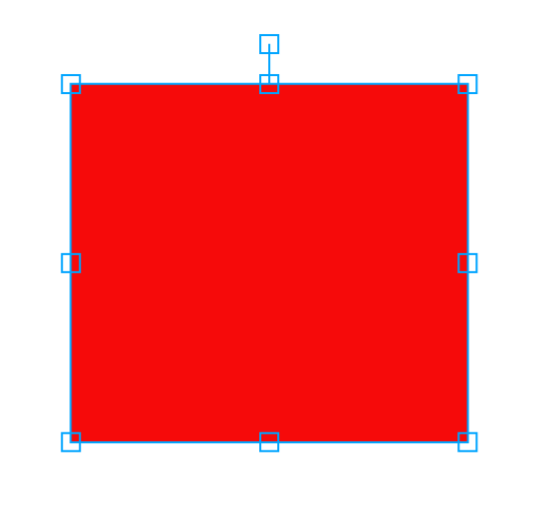
\includegraphics[width=0.9\textwidth]{images/fabric-object-selection}}
		\caption{Manipulácia s objektom}
		\label{img:fabric-object-selection}
	\end{subfigure}
	\quad
	\begin{subfigure}[b]{0.48\linewidth}	
		\centering{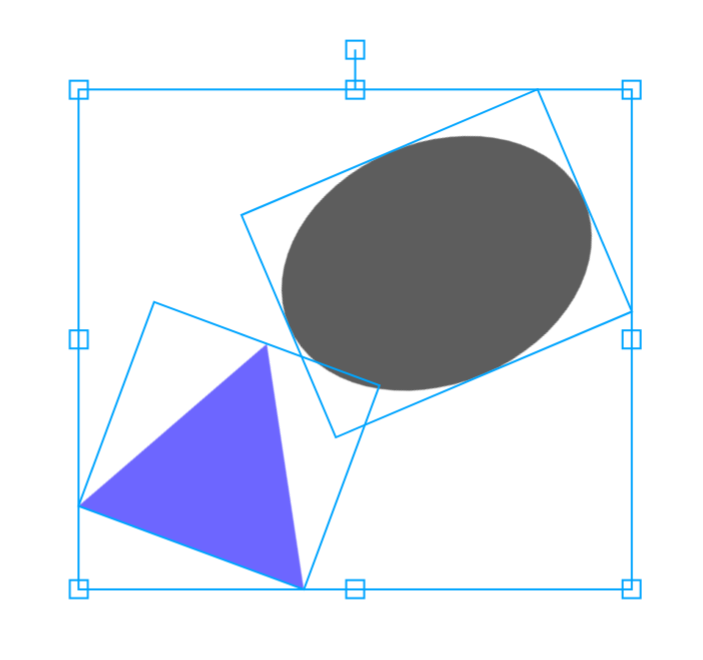
\includegraphics[width=0.9\textwidth]{images/fabric-group-selection}}
		\caption{Manipulácia skupiny objektov}
		\label{img:fabric-group-selection}
	\end{subfigure}
	\caption[Fabric - ukážka manipulácie s objektami]{Manipulácia s objektami pomocou vstupných zariadení s použitím knižnice Fabric}
\end{figure}
\FloatBarrier

\subsubsection{Event}

Aplikácie a frameworky postavené na architektúre riadenej udalosťami poskytujú veľkú flexibilitu a výkonnosť. Knižnica Fabric nie je výnimkou a poskytuje rozšíriteľný systém udalostí (\textit{event}-ov), začínajúc od jednoduchých (spúšťaných akciami počítačovej myši), až po zložité objektové udalosti. Dovoľujú nám odchytávať rôzne akcie odohrávajúce sa v \textit{canvas} grafickej ploche. API na prácu s udalosťami je veľmi jednoduché na obsluhu. Je podobné štandardom implementovaným v jQuery, Underscore.js alebo iných populárnych JavaScriptových knižniciach. Na inicializovanie event listener-u slúži metóda \code{on}\reflst{lst:fabric-events} a na prípadné odstránenie použijeme metódu \code{off}.
\begin{lstlisting}[style=web,caption={Ukážka programovej implementácie na prácu s eventami},captionpos=b, label={lst:fabric-events}]
var canvas = new fabric.Canvas('...');
canvas.on('mouse:down', function(options) {
	console.log('Klikli ste na pozíciu: ', options.e.clientX, options.e.clientY);
	if (options.target) {
		console.log('Klikli ste na objekt: ', options.target.type);
	}
});
\end{lstlisting}
Ako je možné vidieť z ukážky programového kódu vyššie, metóda \code{on} obsahuje dva parametre. Prvým je názov udalosti ktorú chceme odchytávať, tým druhým je metóda spracovávajúca danú udalosť nazývaná \textit{event handler}. Tá prijíma objekt \textit{options}. V tomto objekte sa nachádzajú dve premenné:
\begin{itemize}
	\item \code{e} - originálny JavaScriptový event
	\item \code{target} - objekt na ktorý bolo kliknuté alebo hodnota \code{null}
\end{itemize}
Existuje viacero kategórií udalostí vyvolávaných nasledovnými akciami:
\begin{itemize}
	\item akcie počítačovej myši - \code{mouse:up}, \code{mouse:down}, \code{mouse:move}, \code{mouse:dblclick}, \code{mouse:wheel}, \code{mouse:over}, \code{mouse:out}
	\item akcie zmeny označenia objektu - \code{before:selection:cleared}, \code{selection:cleared}, \code{selection:created}, \code{selection:updated}
	\item akcie objektu - \code{object:added}, \code{object:removed}, \code{object:modified}, \code{object:moving}, \code{object:scaling}, \code{object:rotating}, \code{object:skewing}
	\item akcie grafickej plochy - \code{after:render}
\end{itemize}
Udalosti sú vyvolávané automaticky v rámci programového kódu knižnice Fabric. V prípade že potrebujeme manuálne vyvolať niektorú z udalostí, docielime to pomocou metódy \code{canvas.trigger(...)} \reflst{lst:fabric-trigger}

\begin{lstlisting}[style=web,caption={Manuálne vyvolanie udalosti v knižnici Fabric},captionpos=b, label={lst:fabric-trigger}]
canvas.trigger('object:modified', {target: object});
\end{lstlisting}


\subsection{JavaScriptová knižnica Socket.io}
Socket.IO je JavaScriptová knižnica vytvorená pre realtime webové aplikácie. Socket.IO umožňuje real-time obojstrannú komunikáciu medzi webovým klientom a servermi. Socket.IO má dve časti:
\begin{itemize}
	\item \textit{klientská strana} bežiaca vo webovom prehliadači používateľa
	\item \textit{serverovú strana} pre Node.js aplikáciu riadiacu správanie všetkých klientov
\end{itemize}
Obe časti majú takmer identické API. Podobne ako node.js je socket.io "\textit{event-driven}", teda funkcionalita je vyvolávaná pomocou definovaných funkcií pri určitých akciach používateľa alebo systému.



\section{Rozšírenia MediaWiki (Extensions)}
MediaWiki, tak ako aj množstvo ďalších systémov na správu obsahu stránok, poskytuje spôsob, pomocou ktorého je možné zmeniť správanie aj vzhľad MediaWiki aplikácie. V závislosti od potreby existuje niekoľko kategórií rozšírení (angl.: \textit{extension}):
\begin{itemize}
	\item \textit{Parser extension}: rozšírenie wiki-textu o vlastné značky a príkazy.
	\item \textit{Special page extension}: pridanie funkcionality na reportovanie a administratívu.
	\item \textit{User interface extension}: zmena vzhľadu MediaWiki aplikácie.
	\item \textit{Authentication and Authorisation extension}: rozšírenie zabezpečenia a overenia používateľov pomocou vlastných mechanizmov.
\end{itemize} 

Môžu byť do systému inštalované iba s administrátorským prístupom do súborového systému na serveri. Inštalácia pozostáva zo skopírovania zdrojových súborov do adresára \code{$ \$ $IP\/extensions\/nazov_rozsirenia\/}. Následne ho je možné inicializovať v koreňovom adresári MediaWiki inštalácie, v súbore \code{LocalSettings.php}, pomocou globálnej funkcie
\\
\code{wfLoadExtension(\'nazov_rozsirenia\')}.

Okrem existujúcich oficiálnych rozšírení spravovaných komunitou vývojárov, je možné nainštalovať aj rozšírenia tretích strán. Môže tu však nastať viacero problémov. Dané rozšírenie môže spôsobovať chyby, prípadne úplnú nefunkčnosť aplikácie, nemusí byť viac podporované vývojármi alebo môže byť nekompatibilné s aktuálnou verziou MediaWiki inštalácie. Ak rozšírenie ovplyvňuje štruktúru databázy, je dobré pred inštaláciou previesť proces jej kompletného zálohovania. Pri vývoji vlastného rozšírenia je preto potrebné myslieť na tieto faktory a snažiť sa dodržiavať konvencie programovania pre systém MediaWiki \cite{MediaWikiConventions}. 

Pre správne fungovanie rozšírenia je potrebné zabezpečiť niekoľko kľúčových vlastností, pozostávajúcich z týchto krokov:
\begin{itemize}
	\item Zaregistrovať akýkoľvek media handler, parsovaciu funckiu, špeciálne stránky, vlastné XML značky a premenné použité vašim rozšírením.
	\item Definovať a zvalidovať každú konfiguračnú premennú.
	\item Pripraviť triedy použité vo vašom rozšírení pre autonačítanie.
	\item Rozhodnúť ktoré časti inštalačného nastavenia majú byť vykonané okamžite a ktorá majú čakať pokiaľ sa inicializuje jadro MediaWiki.
	\item Definovať dodatočné hooky potrebné pre rozšírenie.
	\item Vytvoriť / skontroluje všetky nové databázové tabuľky nutné pre rozšírenie.
	\item Nastaviť lokalizáciu rozšírenia.
\end{itemize}

\subsection{ResourceLoader}
Vytváraním rozšírení existujúcich systémov vzniká množstvo súborov, odosielaných zo servera na jednotlivých klientov. Aby sa predišlo dlhému načítaniu stránky, je potrebné nejakým spôsobom riadiť, kedy a komu sa majú odoslať zdrojové súbory. Systém MediaWiki na to využíva takzvaný \textit{delivery system} označovaný taktiež ako \textit{ResourceLoader}. Jeho úlohou je odosielať zdrojové súbory, ktoré klientská časť aplikácie aktuálne potrebuje a ktoré podporuje internetový prehliadač klienta. Využíva pri tom nasledujúce procesy:

\begin{itemize}
	\item \textit{Minifikácia a spájanie} zdrojových súborov optimalizuje ich veľkosť a tým pádom aj redukuje čas ich načítania.
	\item \textit{Dávkové načítavanie} viacerých modulov (rozšírení) súčasne s použitím predchádzajúceho procesu minifikácie a spájania redukuje počet dopytov na server.
	\item \textit{Data URI embedovanie} zdrojových obrázkov v kaskádových štýloch taktiež redukuje počet potrebných dopytov na server a tým aj jeho čas odozvy.
\end{itemize}